% -*- mode: latex; -*- mustache tags:  
\documentclass[10pt,twoside,english]{_support/latex/sbabook/sbabook}
\let\wholebook=\relax

\usepackage{import}
\subimport{_support/latex/}{common.tex}

%=================================================================
% Debug packages for page layout and overfull lines
% Remove the showtrims document option before printing
\ifshowtrims
  \usepackage{showframe}
  \usepackage[color=magenta,width=5mm]{_support/latex/overcolored}
\fi


% =================================================================
\title{Learning Object-Oriented Programming, Design and TDD with Pharo}
\author{Stéphane Ducasse}
\series{The Pharo TextBook Collection}

\hypersetup{
  pdftitle = {Learning Object-Oriented Programming, Design and TDD with Pharo},
  pdfauthor = {Stéphane Ducasse},
  pdfkeywords = {Introduction, programming, design, testing, Pharo, Smalltalk}
}


% =================================================================
\begin{document}

% Title page and colophon on verso
\maketitle
\pagestyle{titlingpage}
\thispagestyle{titlingpage} % \pagestyle does not work on the first one…

\cleartoverso
{\small

  Copyright 2017 by Stéphane Ducasse.

  The contents of this book are protected under the Creative Commons
  Attribution-ShareAlike 3.0 Unported license.

  You are \textbf{free}:
  \begin{itemize}
  \item to \textbf{Share}: to copy, distribute and transmit the work,
  \item to \textbf{Remix}: to adapt the work,
  \end{itemize}

  Under the following conditions:
  \begin{description}
  \item[Attribution.] You must attribute the work in the manner specified by the
    author or licensor (but not in any way that suggests that they endorse you
    or your use of the work).
  \item[Share Alike.] If you alter, transform, or build upon this work, you may
    distribute the resulting work only under the same, similar or a compatible
    license.
  \end{description}

  For any reuse or distribution, you must make clear to others the
  license terms of this work. The best way to do this is with a link to
  this web page: \\
  \url{http://creativecommons.org/licenses/by-sa/3.0/}

  Any of the above conditions can be waived if you get permission from
  the copyright holder. Nothing in this license impairs or restricts the
  author's moral rights.

  \begin{center}
    
\includegraphics[width=0.2\textwidth]{_support/latex/sbabook/CreativeCommons-BY-SA.pdf}
  \end{center}

  Your fair dealing and other rights are in no way affected by the
  above. This is a human-readable summary of the Legal Code (the full
  license): \\
  \url{http://creativecommons.org/licenses/by-sa/3.0/legalcode}

  \vfill

  % Publication info would go here (publisher, ISBN, cover design…)
  Layout and typography based on the \textcode{sbabook} \LaTeX{} class by Damien
  Pollet.
}


\frontmatter
\pagestyle{plain}

\tableofcontents*
\clearpage\listoffigures

\mainmatter

\chapter{Beacons and Satellites }\label{ch:beacon}
In this chapter you will build a simulator for beacons and satellites. Beacons are in the sea and collect data and from time to time they should synchronise with satelittes to send data. 

In reality, satelittes broadcast signals and beacons are polling at regular interval for signals, then once they know that they are in range based on the first signal, a communication is established and data is exchanged.

In the simulator we will present how we can implement communication between losely coupled objects. You will build step by step different variations around the observer/observable idiom. This idiom is important since it is used in Model-View-Controller and Self addressed stamped enveloppe (S.A.S.E) patterns. Beacons will register to satellites and when the satelittes are in range they will notify the beacons interested in the notification. 
\section{Description}

\begin{figure}

\begin{center}
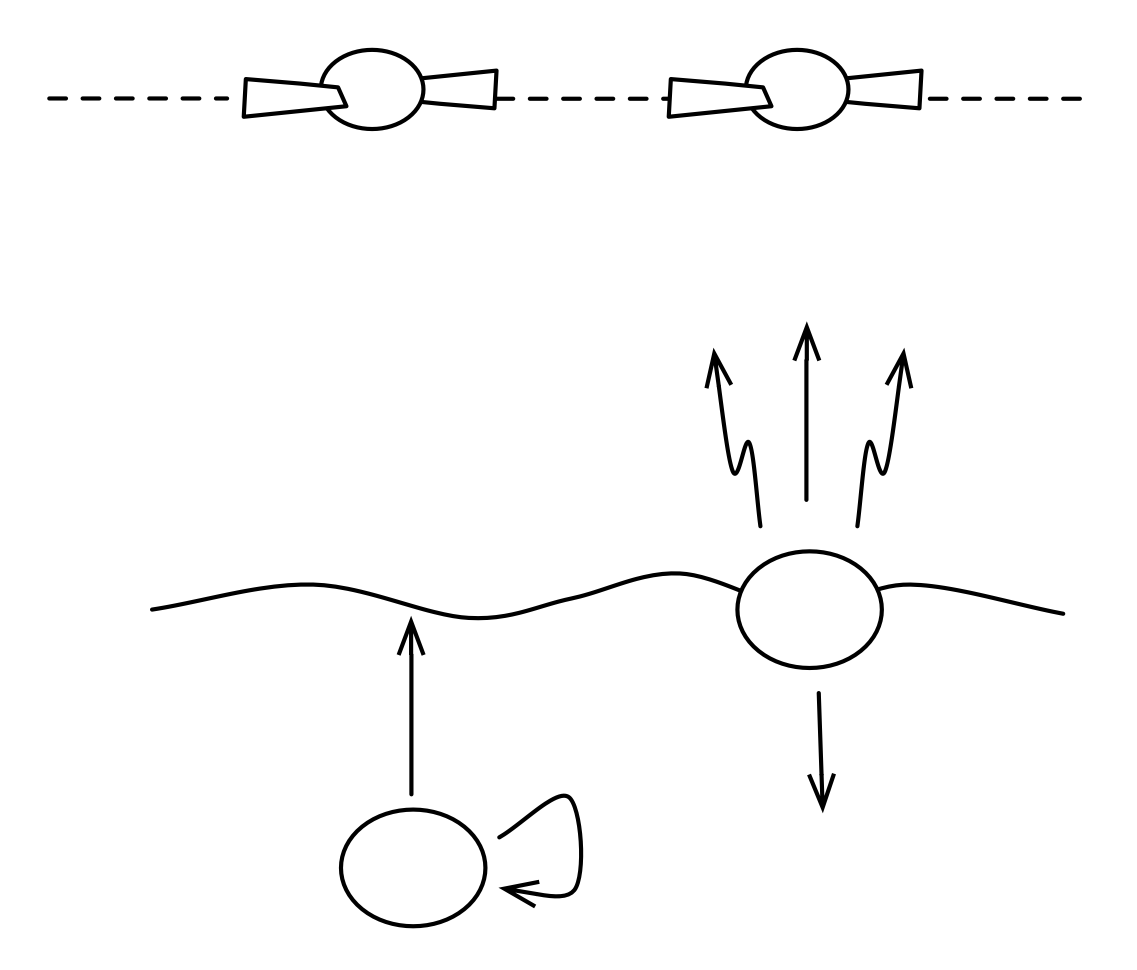
\includegraphics[width=0.7\textwidth]{/Users/ducasse/Workspace/FirstCircle/MyBooks/Bk-Writing/PharoBooks/LearningOOPWithPharoTrans/_result/pdf/Chapters/BeaconAndSatellite/figures/Beacons.png}\caption{Beacons and Satelittes.\label{fig:Beacon}}\end{center}
\end{figure}


A beacon is inside the sea and it collects data. It is fully autonomous. After a certain period of time it migrates to the surface waiting to send the data it collected.
To communicate with satelittes, a satelitte should be available, i.e., within the zone where the beacon is.

A satellite is moving around earth at a certain speed and ranging a portion of sea. 
It can only communicate with beacons within such range.

The system is fully dynamic in the sense that new beacons may be added or removed.
Satelittes may be present or not.
\section{A simple model}
\begin{displaycode}{plain}
Object subclass: #Satelitte
	instanceVariableNames: 'observers'
	classVariableNames: ''
	package: 'SatelitteAndBeacon'
\end{displaycode}

\begin{displaycode}{plain}
Satelitte >> initialize
	observers := OrderedCollection new
\end{displaycode}

\begin{displaycode}{plain}
Object subclass: #Beacon
	instanceVariableNames: 'data'
	classVariableNames: ''
	package: 'SatelitteAndBeacon'
\end{displaycode}
\section{V1: Simple observer / observable}
We start with a simple schema where beacons 

\begin{itemize}
\item register to satellites and
\item when the satelittes are in range they notify the beacons that registered.
\end{itemize}
\subsection{Registration}
A beacon register to a satellite as follows:

\begin{displaycode}{plain}
Satelitte >> register: aBeacon
	self addObserver: aBeacon
\end{displaycode}
\subsection{Notification}
\begin{displaycode}{plain}
Satelitte >> position: aPoint
	position := aPoint. 
	self notify
\end{displaycode}

\begin{displaycode}{plain}
Satelitte >> notify
	observers do: [ :aBeacon | aBeacon salelittePositionChanged: self ]
\end{displaycode}
\section{V1 Implementation}
???
\section{V2: Analysis}
This first implementation has several drawbacks.

\begin{itemize}
\item One of the problem is that the message is hardcoded. 
\item Second Imagine that the satellite should emit different notification for its position, protocol to be used, frequency.... and each kind of beacon can register for the notification kinds that fits it. We must have a list of each kind of observed property.
\end{itemize}
\section{V2: Introducing events}
\begin{displaycode}{plain}
Satelitte >> register: aBeacon forEvent: aEventClass
	aSatelitte1 addObserver: aBeacon1 with: aEventClass
\end{displaycode}

\begin{displaycode}{plain}
Satelitte >> addObserver: anObserver with: anEventClass
	observerDict at: anEventClass iAbsentPut: [OrderedCollection new].
	(observerDict at: anEventClass) add: anObserver
\end{displaycode}

\begin{displaycode}{plain}
Satelitte >> position: aPoint
	position := aPoint. 
	self notify: (PositionChanged with: self)
\end{displaycode}

\begin{displaycode}{plain}
Satelitte >> notify: anEvent
	(observersDict at: anEvent class) ifPresent: [ :aBeaconList | 
		aBeaconList do: [:aBeacon| anEvent fireOn: aBeacon ]
\end{displaycode}
\subsection{Implementation}
\begin{displaycode}{plain}
Object subclass: #SBEvent
	instanceVariableNames: 'observable'
	classVariableNames: ''
	package: 'SatelitteAndBeacon'
\end{displaycode}

\begin{displaycode}{plain}
SBEvent subclass: #SBPositionChanged
	instanceVariableNames: ''
	classVariableNames: ''
	package: 'SatelitteAndBeacon'
\end{displaycode}

\begin{displaycode}{plain}
SBEvent subclass: #SBProtocolChanged
	instanceVariableNames: ''
	classVariableNames: ''
	package: 'SatelitteAndBeacon'
\end{displaycode}

\begin{displaycode}{plain}
SBPositionChanged >> fireOn: anObserver
	anObserver salelittePositionChanged: observable
\end{displaycode}

\begin{displaycode}{plain}
SBProtocolChanged >> fireOn: anObserver
	anObserver salelitteProtocolChanged: observable
\end{displaycode}
\subsection{V2 analysis}
Advantages

\begin{itemize}
\item we reuse the same mechanism for different kind of observable properties.
\end{itemize}

Drawbacks

\begin{itemize}
\item One event means that the message is also hardcoded. There is tight dependencies between  the event type and the kind of behavior that is available on the observer side. 
\end{itemize}
\section{V3 Specifying the message}
Now the observer can specify the message that it wants to receive. 

\begin{displaycode}{plain}
aSatelitte1 when: SBPositionChanged send: #readyForHandShakeWith: to: aBeacon1
\end{displaycode}

\begin{displaycode}{plain}
aSatelitte1 when: SBProtocolChanged send: #useProtocol: to: aBeacon1
\end{displaycode}

\begin{displaycode}{plain}
Satelitte >> when: anEventClass send: aSelector to: anObserver
	observerDict at: anEventClass iAbsentPut: [OrderedCollection new].
	(observerDict at: anEventClass) add: (aSelector -> anObserver)
\end{displaycode}

\begin{displaycode}{plain}
Satelitte >> position: aPoint
	position := aPoint. 
	self notify: (PositionChanged with: self)
\end{displaycode}

\begin{displaycode}{plain}
Satelitte >> notify: anEvent
	(observersDict at: anEvent class) ifPresent: [ :aBeaconList | 
		aBeaconList do: [ :aBeaconAssoc | 
			aBeaconAssoc value perform: aBeaconAssoc key with: anEvent) ]
\end{displaycode}
\section{V5 Factoring out the announcer}
The notification and management at notification should be packaged as a separate class so that we can reuse it by just delegating to it. 

\begin{displaycode}{plain}
Object subclass: #BSAnnouncement
	instanceVariableNames: 'selector observer'
\end{displaycode}

\begin{displaycode}{plain}
Object subclass: #BSAnnouncer
	instanceVariableNames: 'observerDict'
\end{displaycode}

\begin{displaycode}{plain}
BSAnnouncer >> when: anEventClass send: aSelector to: anObserver
	observerDict at: anEventClass iAbsentPut: [ OrderedCollection new] .
	(observerDict at: anEventClass) add: 
		(BSAnnouncement send: aSelector to: anObserver)
\end{displaycode}

\begin{displaycode}{plain}
BSAnnouncer >> notify: anEvent
	(observersDict at: anEvent class) ifPresent: [ :aBeaconList | 
		aBeaconList do: [ :anAnnouncement | 
			anAnnouncement observer
				perform: anAnnouncement selector 
				with: anEvent) ]
\end{displaycode}

\begin{displaycode}{plain}
Satelitte >> notify: anEvent
	self announcer notify: anEvent
\end{displaycode}

\begin{displaycode}{plain}
Satelitte >> when: anEventClass send: aSelector to: anObserver
	self announcer when: anEventClass send: aSelector to: anObserver
\end{displaycode}
\section{Discussion about lookup of events}

% lulu requires an empty page at the end. That's why I'm using
% \backmatter here.
\backmatter

% Index would go here
\bibliographystyle{abbrv}
\bibliography{others.bib}
\end{document}
